Figure \ref{PositioningMap} on the next page shows my recommendation for the best consumer positioning for MUJI in relation to the target group. I will use the 4 P's\footnote{Product, Place, Promotion, Price} in the following section to quickly outline how MUJI should define their marketing mix in order to differentiate themselves from the competitors.  
\\\\
\textbf{Product}. Simple, functional, minimalist and good quality products with no labels, meeting the demands of the young agnostic shoppers. 

\textbf{Price}. Low- to mid-price. This parameter is elaborated in chapter \ref{Chapter3}.

\textbf{Place (distribution)}. Bricks and mortar shop in Copenhagen. Furthermore, the webshop should be prioritised highly, because of the increase in consumer expenditure online. From 2014 - 2018 online sales are expected to increase with 27,7\% in Denmark \cite[5]{ConsumerLifestyles}. 

\textbf{Promotion}. Authenthic, inspirational and not-pushy campaigns and material reaching the target group through social media, story telling and exhibitions. 

\begin{figure}[H]
    \centering
    \caption{Positioning map (\ref{Competitors})}
    \label{PositioningMap}
    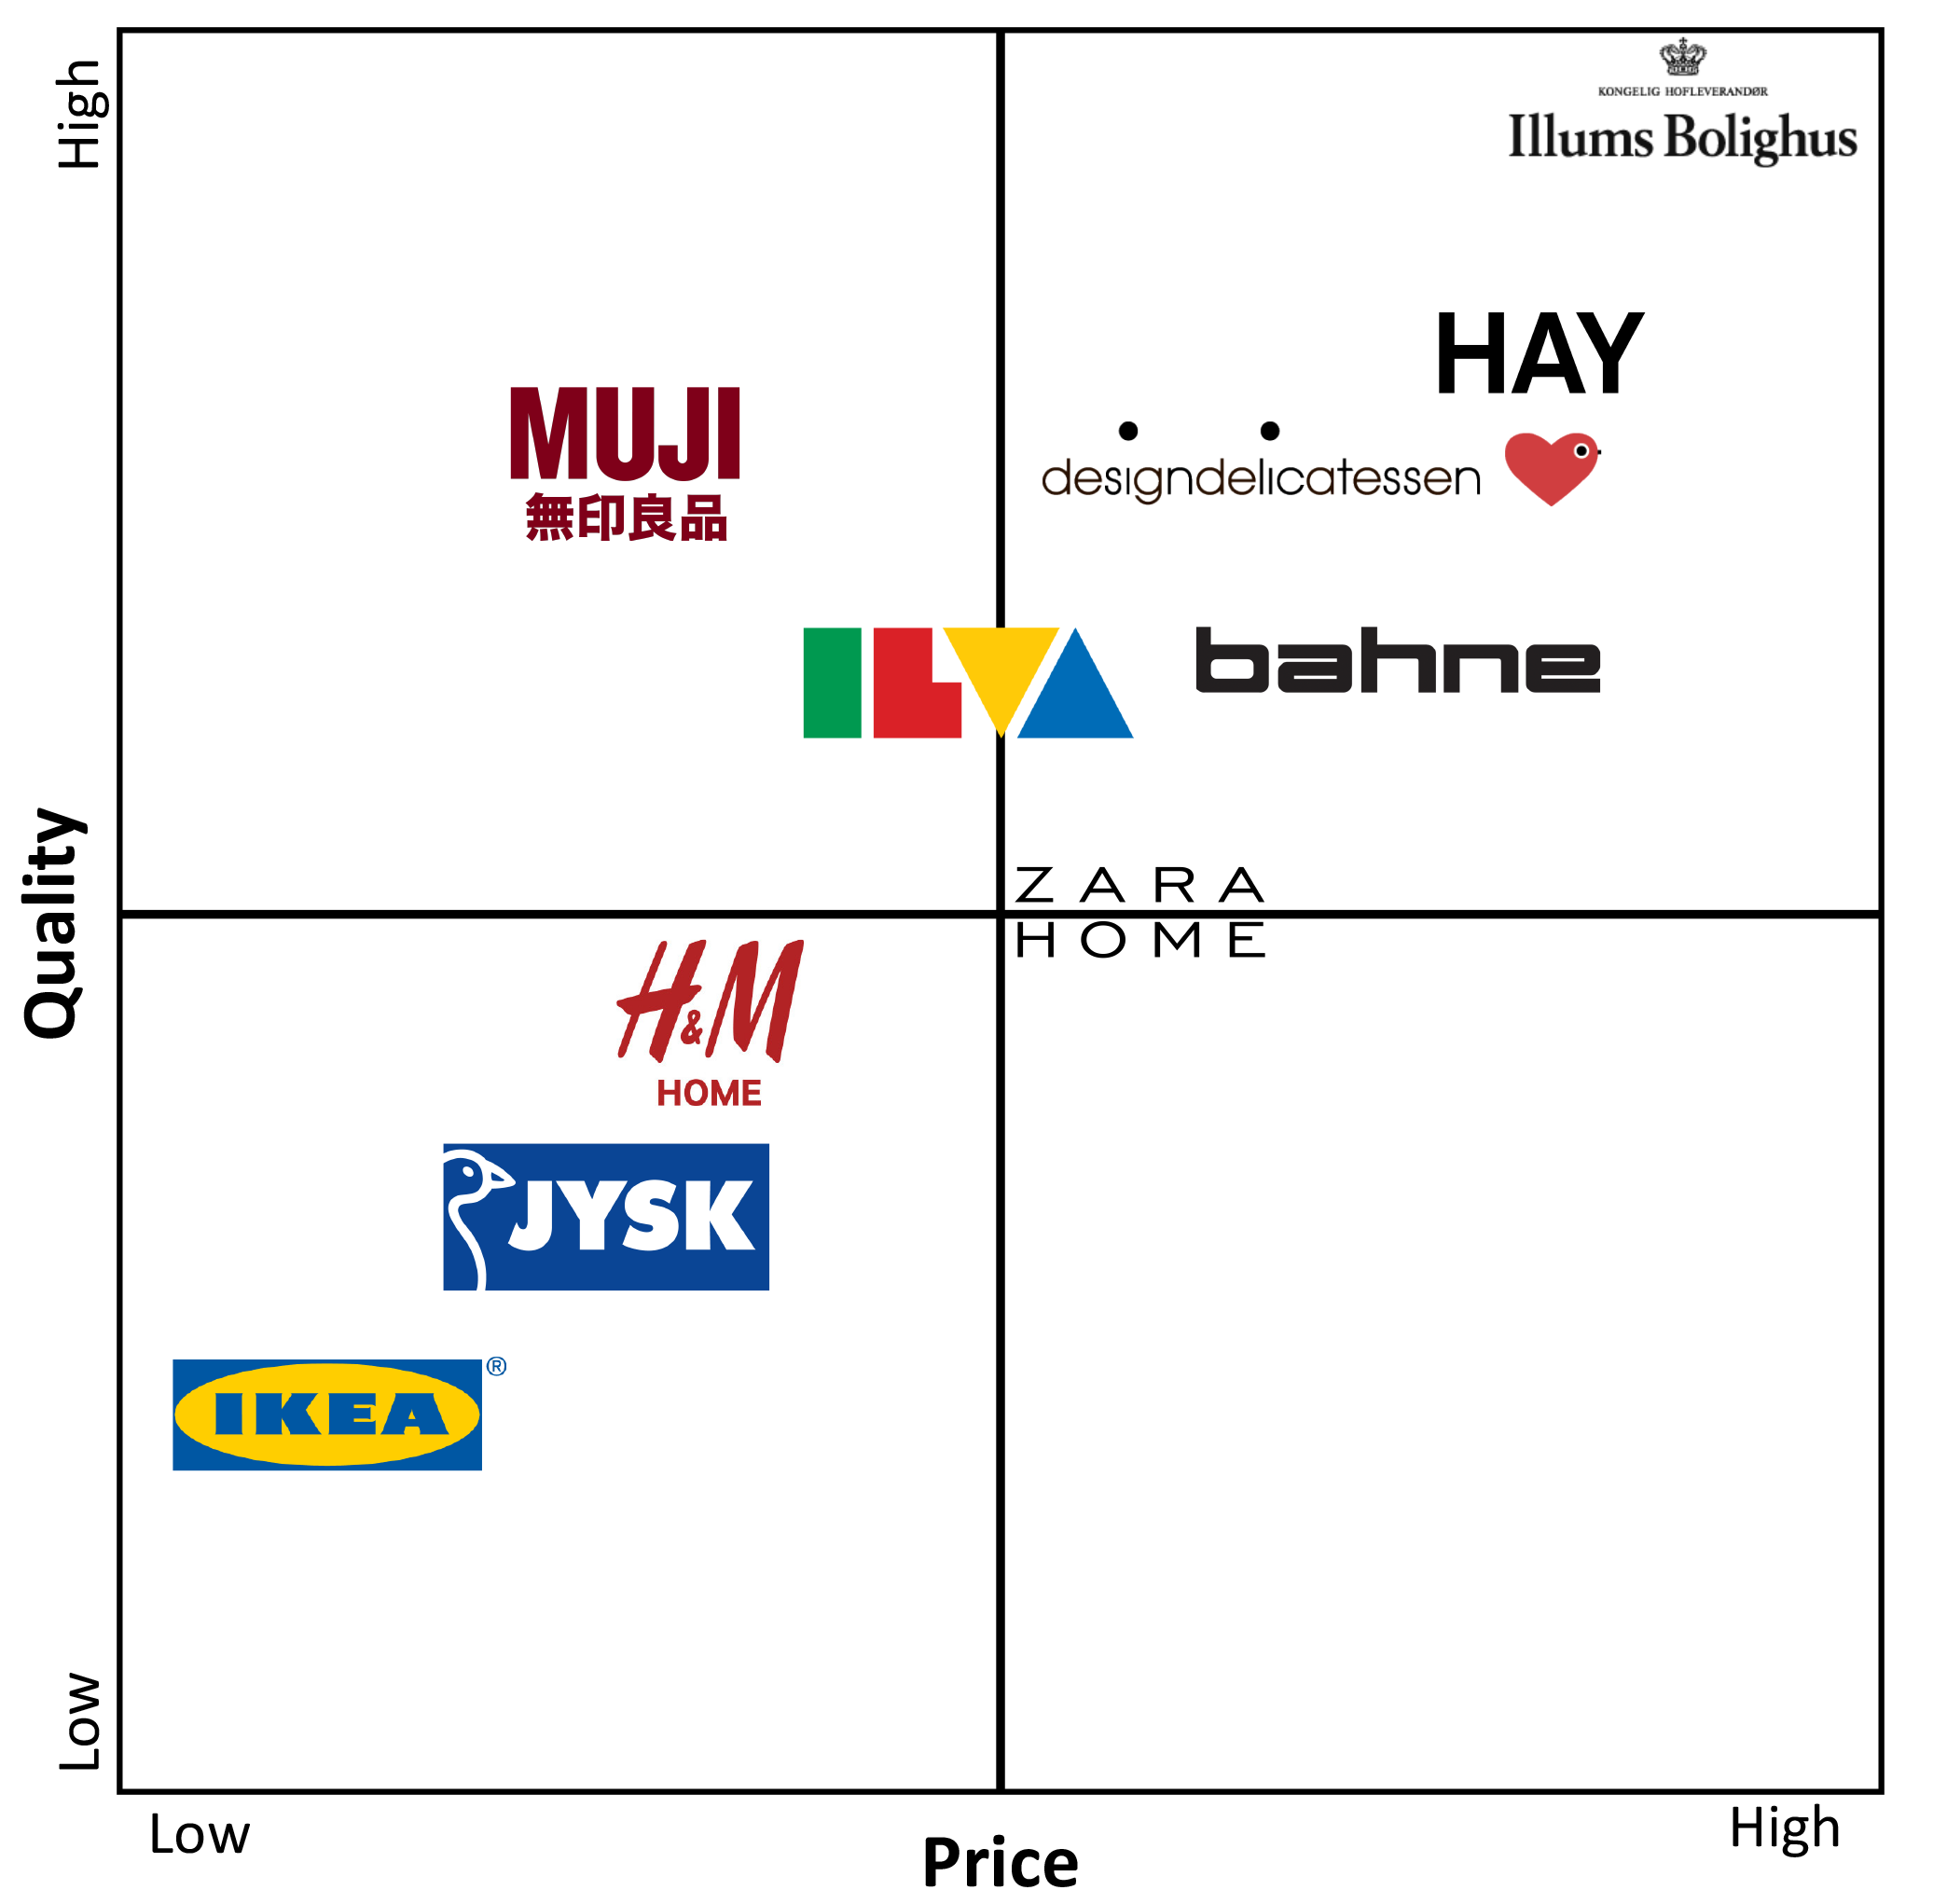
\includegraphics[width=12 cm]{ConsumerPositioning/CompetitionMapV3.png}
\end{figure}

